\chapter{Конструкторская часть}
В данном разделе будут рассмотрены схемы алгоритмов сортировок, а также найдена их трудоемкость.

\section{Требования к ПО}
Ряд требований к программе:
\begin{itemize}
	\item на вход подается массив целых чисел в диапазоне от -10000 до 10000;
    \item возвращается отсортированный по возрастанию массив, который был задан в предыдущем пункте. \newline
\end{itemize}

\section{Разработка алгоритмов}
На рисунках \ref{fig:comb}-\ref{fig:merge2} представлены схемы алгоритмов сортировки - расческой, бинарным деревом и слиянием.

\begin{figure}[h!]
	\centering
	\includegraphics[width=0.8\linewidth]{img/comb}
	\caption{Схема алгоритма сортировки расческой}
	\label{fig:comb}
\end{figure}
\begin{figure}[h!]
	\centering
	\includegraphics[width=0.8\linewidth]{img/bin_tree}
	\caption{Схема алгоритма сортировки бинарным деревом - 1 часть}
	\label{fig:bin_tree}
\end{figure}
\begin{figure}[h!]
	\centering
	\includegraphics[width=0.8\linewidth]{img/bin_tree2}
	\caption{Схема алгоритма сортировки бинарным деревом - 2 часть}
	\label{fig:bin_tree2}
\end{figure}
\begin{figure}[h!]
	\centering
	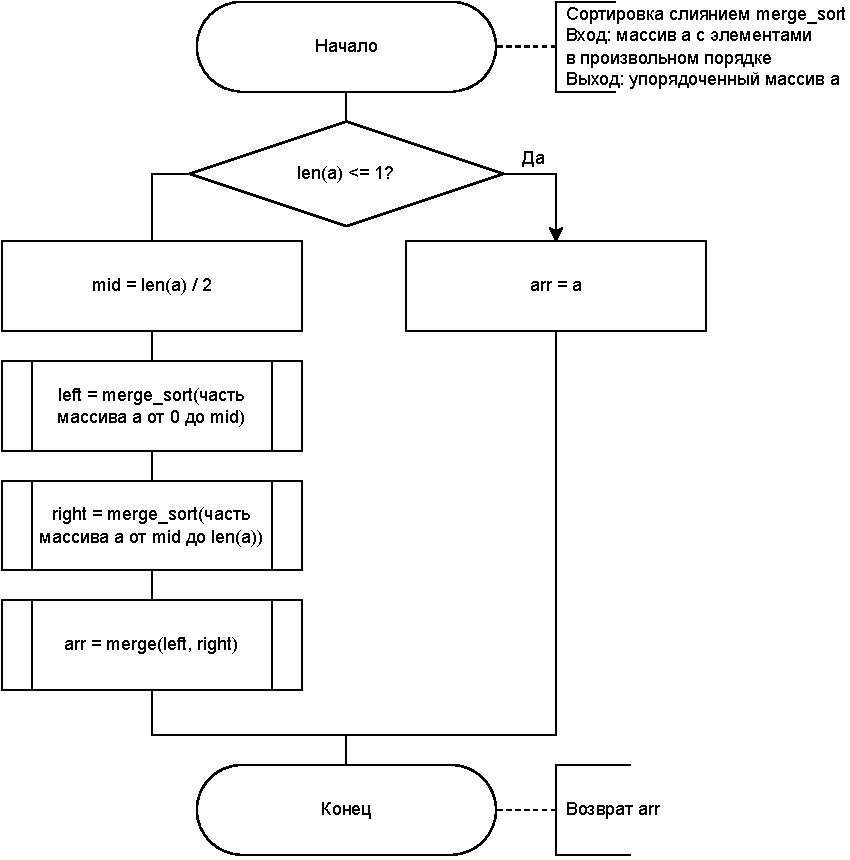
\includegraphics[width=0.8\linewidth]{img/merge}
	\caption{Схема алгоритма сортировки слиянием - 1 часть}
	\label{fig:merge}
\end{figure}

\begin{figure}[h!]
	\centering
	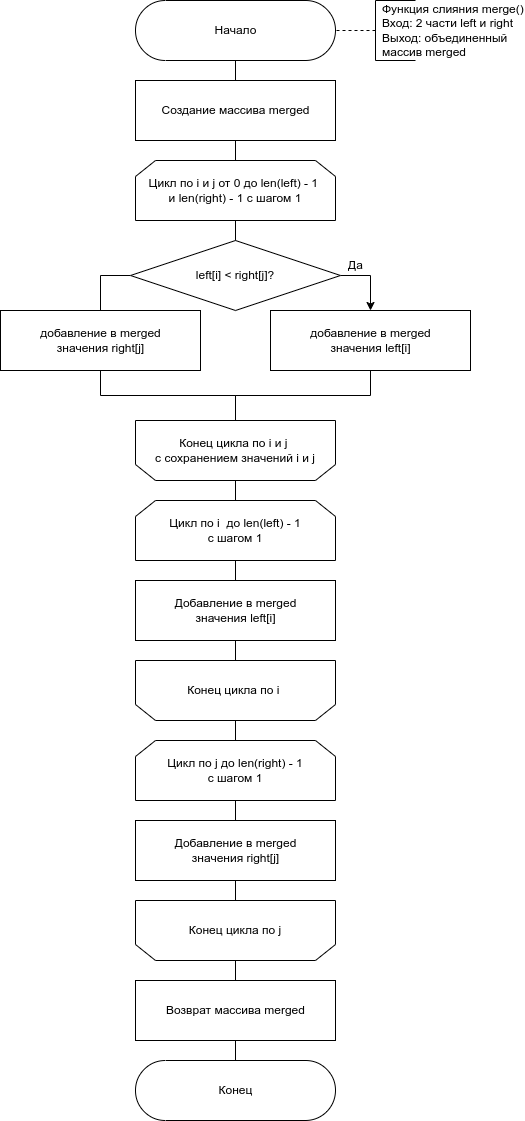
\includegraphics[width=0.7\linewidth]{img/merge2}
	\caption{Схема алгоритма сортировки слиянием - 2 часть}
	\label{fig:merge2}
\end{figure}

\clearpage

\section{Модель вычислений для проведения оценки трудоемкости}
Чтобы провести вычисление трудоемкости алгоритмов умножения матриц, введем модель вычислений \cite{model}:

\begin{enumerate}[label=\arabic*)]
	\item Трудоемкость следующих базовых операций единична:
	+, -, =, +=, -=, ==, !=, <, >, <=, >=, [], ++, --, <<, >>.
	Операции *, \%, / имеют трудоемкость 2.
	\item трудоемкость оператора выбора \code{if условие then A else B} рассчитывается, как (\ref{for:if});
	\begin{equation}
		\label{for:if}
		f_{if} = f_{\text{условия}} +
		\begin{cases}
			f_A, & \text{если условие выполняется,}\\
			f_B, & \text{иначе.}
		\end{cases}
	\end{equation}
	\item трудоемкость цикла рассчитывается, как (\ref{for:for});
	\begin{equation}
		\label{for:for}
		f_{for} = f_{\text{инициализации}} + f_{\text{сравнения}} + N(f_{\text{тела}} + f_{\text{инкремента}} + f_{\text{сравнения}})
	\end{equation}
	\item трудоемкость передачи параметров в функцию и возврат из нее равны 0.
\end{enumerate}


\section{Трудоёмкость алгоритмов}

Определим трудоемкость выбранных алгоритмов сортировки. Введем обозначение $N$ - количество элементов в массиве.

\subsection{Алгоритм сортировки расческой}

Трудоемкость сортировки расческой состоит из:
\begin{enumerate}
	\item[1)] предварительных расчетов трудоемкостью (\ref{for:k2});
	\begin{equation}
		\label{for:k2}
		f(N) = 3
	\end{equation}
	\item[2)] цикла, трудоемкость которого равна (\ref{for:k1}), где $t$ --- фактор, в нашем случае 1.247. 
	\begin{equation}
		\label{for:k1}
		f(N) = 1 + log_t(N) \cdot (1 + 2 + 9N + 1) + 2
	\end{equation}
\end{enumerate}

Трудоемкость при лучшем случае (отсортированный массив) определяется формулой (\ref{for:t1}).
\begin{equation}
	\label{for:t1}
	f(N) = log_t(N) \cdot (4 + N) + 3
\end{equation}

Однако стоит учитывать, что при факторе $\approx$ 1.3, трудоемкость аппроксимируется как в формуле (\ref{for:t2}), где $C$ --- некая константа. 
\begin{equation}
	\label{for:t2}
	log_t(N) \cdot (4 + N) + 3 \approx C \cdot log(N) \cdot N \approx O(N \cdot log(N))
\end{equation}

Трудоемкость при худшем случае (\ref{for:t4}).
\begin{equation}
	\label{for:t4}
	f(N) =log_t(N) \cdot (4 + 9N) + 3 \approx O(N^2)
\end{equation}

\subsection{Алгоритм сортировки бинарным деревом}

Трудоемкость алгоритма сортировки бинарным деревом состоит из:
\begin{enumerate}[label=\arabic*)]
	\item Трудоемкости построения бинарного дерева, которая равна (\ref{for:make_tree});
	\begin{equation}
		\label{for:make_tree}
		f_{make\_tree} = (5 \cdot \log(N) + 3) * N = N \cdot \log(N)
	\end{equation}
	\item Трудоемкости восстановления порядка элементов массива, которая равна (\ref{for:make_arr}).
	\begin{equation}
		\label{for:make_arr}
		f_{main\_loop} = 7 N
	\end{equation}
\end{enumerate}

Таким образом общая трудоемкость алгоритма выражается как (\ref{for:been_total}).
\begin{equation}
	\label{for:been_total}
	f_{total} = f_{make\_tree} + f_{main\_loop}
\end{equation}


Для наилучшего и наихудшего случая общая трудоемкость алгоритма совпадает и равна (\ref{for:been}).
\begin{equation}
	\label{for:been}
	f = O(N\log(N))
\end{equation}



\subsection{Алгоритм сортировки слиянием}

Трудоемкость алгоритма сортировки слиянием состоит из трудоемкости функций $merge$ и $merge\_sort$.

Трудоемкость функции merge состоит из
\begin{enumerate}[label=\arabic*)]
	\item предварительной инициализации, трудоемкость которой равна 2;
	\item основного цикла, трудоемкость которого (\ref{for:main_loop});
	\begin{equation}
		\label{for:main_loop}
		f_{main\_loop} = 2 + N\cdot(3 + 8)
	\end{equation}
	\item 2 дополнительных циклов, трудоемкость которых (\ref{for:extra_loop})
	\begin{equation}
		\label{for:extra_loop}
		f_{extra\_loop} = (k_1 + k_2)\cdot6
	\end{equation}
	где $k_1 < N/2$ и $k_2 < N/2$.
	
	Общая трудоемкость:  $2 + 2 + N * (3 + 8) + (k1 + k2) * 6 = 11N + 4  + 6(k1 + k2) = O(N)$, где $k1 < N/2, k2  < N/2$
\end{enumerate}

Вычислим трудоемкость $merge\_sort$. Разобьём все “слияния”, выполненные в процессе сортировки массива на “слои”. Слияние двух частей изначального массива - первый слой, слияния частей каждой из этих двух частей (четвертей оригинального массива) - второй слой, и т.д. Необходимо заметить, что количество элементов в каждом слое равна $N$. Тогда на каждом слое все слияния выполняются за $O(N)$. Известно, что количество таких строк, называемое глубиной рекурсивного дерева, будет $log(N)$.

Для наилучшего и наихудшего случая общая сложность mergeSort совпадает и равна: $O(N * log(N))$ \cite{algos}.


\section*{Вывод}

Были разработаны схемы всех трех алгоритмов сортировки. Также для каждого из них были рассчитаны и оценены лучшие и худшие случаи.
